% LangClaw — JAIIO 2025/2026 submission (full paper, max 14 pages)
% Uses LNCS class (llncs.cls) as required by JAIIO guidelines.
% Anonymous submission: author/institute information omitted.
%
\documentclass{llncs}

\usepackage[a4paper, top=5.2cm, bottom=5.2cm, left=4.4cm, right=4.4cm]{geometry}
\usepackage[T1]{fontenc}
\usepackage[utf8]{inputenc}
\usepackage{mathptmx}
\usepackage{graphicx}
\usepackage{float}
\usepackage{amsmath,amssymb}
\usepackage{booktabs}
\usepackage{algorithm}
\usepackage{algpseudocode}
\usepackage{listings}
\usepackage{enumitem}

\setlength{\textfloatsep}{10pt plus 2pt minus 2pt}
\setlength{\floatsep}{8pt plus 2pt minus 2pt}
\setlength{\intextsep}{8pt plus 2pt minus 2pt}
\raggedbottom

\lstset{
  basicstyle=\small\ttfamily,
  breaklines=true,
  frame=single,
  language=Python,
  numbers=none,
  xleftmargin=1em,
  xrightmargin=1em,
}

\usepackage[style=apa]{biblatex}
\addbibresource{references.bib}

\begin{document}

% ============================================================
% ENGLISH TITLE + ABSTRACT + KEYWORDS
% ============================================================
\title{LangClaw: Endogenous Homeostatic Regulation for Mitigating Context
Collapse in Multi-Agent LLM Debate Systems\thanks{Durante la
preparaci\'on de este trabajo, los autores utilizaron GPT-5.4 con el fin
de mejorar el lenguaje y la legibilidad del manuscrito. Tras utilizar
esta herramienta, los autores revisaron y editaron el contenido seg\'un
fue necesario y asumen plena responsabilidad por el contenido de la
publicaci\'on. El detalle completo de tooling de IA empleado en
investigaci\'on, desarrollo e ilustraciones se documenta en el
repositorio del proyecto.}}

% Anonymous submission — authors omitted for review
\author{}
\institute{}

\maketitle

\begin{abstract}
Multi-agent LLM systems tend to lose coherence as interaction extends---a
problem known as \emph{context collapse}. Existing frameworks address this
through static orchestration or periodic heartbeats, but both treat
participation frequency as a design constant. We ask whether it can instead
be an emergent property of each agent's internal regulatory state.
We present LangClaw, a framework grounded in a formal theory of homeostatic
agency in which each agent maintains an epistemic deficit
$\delta_i \in [\varepsilon,\infty)$ governed by a drive function
$D(\delta) = (\delta - \varepsilon)^2$; reward is defined as drive reduction,
implementing the equivalence theorem of Keramati and Gutkin (2014). A
multi-criteria stimulus evaluator acts as sensor; an online Q-learner
with $\varepsilon$-greedy exploration selects actions via TD(0). This
represents a structural departure from the prevailing heartbeat paradigm:
rather than firing on a fixed schedule, agents activate when internal
pressure warrants it and learn which actions most effectively reduce drive.
We evaluate LangClaw against a LangGraph-style LLM router under equal
heartbeat budgets in a zero-sum political debate with ten GPT-5-nano agents
organized as two VSM-inspired factions, measuring discourse structure through
AAF metrics, graph-structural peer reference, and the quality proxy
$\Delta\varphi^*$. Preliminary results show HRRL produces $5\times$ more
debates with higher AAF acceptance, no silenced agents, and improving
structural quality, while LangGraph degrades.

\keywords{multi-agent systems \and large language models \and homeostasis \and
reinforcement learning \and context collapse \and event-driven architecture}
\end{abstract}
\clearpage

% ============================================================
% SPANISH TITLE + RESUMEN + KEYWORDS
% ============================================================
\begin{center}
{\Large \bfseries\boldmath LangClaw: Regulaci\'on Homeost\'atica End\'ogena
para Mitigar el Colapso del Contexto en Sistemas de Debate Multi-Agente
basados en LLM}
\end{center}

\begin{abstract}
Los sistemas multi-agente de LLM tienden a perder coherencia a medida que
la interacci\'on se extiende---un problema conocido como \emph{colapso del
contexto}. Los enfoques actuales---enrutadores, grafos, heartbeats
peri\'odicos---ampliaron capacidades sin alterar un supuesto estructural: la
frecuencia de participaci\'on es un par\'ametro ex\'ogeno, no una propiedad
del agente. Este trabajo propone invertir ese supuesto. Inspirado en el
aprendizaje por refuerzo homeost\'atico (Keramati y Gutkin, 2014), cada
agente mantiene un d\'eficit epist\'emico
$\delta_i \in [\varepsilon,\infty)$ gobernado por $D(\delta)=(\delta-\varepsilon)^2$;
la recompensa es reducci\'on de impulso $r_t = D(\delta_t)-D(\delta_{t+1})$.
Un evaluador multicriterio act\'ua como sensor; un Q-learner con pol\'itica
$\varepsilon$-greedy selecciona acciones v\'ia TD(0). La frecuencia de
participaci\'on no se fija ni se enruta: \emph{emerge}. Evaluamos LangClaw
contra un enrutador al estilo LangGraph en un debate pol\'itico con diez
agentes GPT-5-nano organizados como dos facciones inspiradas en el VSM,
midiendo coherencia argumentativa mediante m\'etricas AAF, PRR$_G$ y
$\Delta\varphi^*$. Resultados preliminares muestran que HRRL produce
$5\times$ m\'as debates con mayor aceptaci\'on AAF, sin agentes
silenciados y con calidad estructural creciente, mientras LangGraph
se degrada.

\keywords{sistemas multi-agente \and modelos de lenguaje \and homeostasis \and
aprendizaje por refuerzo \and colapso del contexto \and arquitectura dirigida
por eventos}
\end{abstract}

\setcounter{page}{1}

% ============================================================
\section{Introducci\'on}
\label{sec:intro}

Los sistemas multiagente basados en LLM comienzan a emplearse en procesos
deliberativos de larga duraci\'on---an\'alisis de pol\'iticas, revisi\'on
cient\'ifica, toma de decisiones institucionales---donde la p\'erdida
de coherencia no queda contenida en el software: una recomendaci\'on
de pol\'itica sostenida sobre un debate internamente viciado puede
afectar a millones o una revisi\'on cient\'ifica basada en premisas
alucinadas contamina la literatura sobre la que se construye m\'as
ciencia ---un problema creciente--- El escalamiento
del c\'omputo en tiempo de inferencia~\parencite{snell2024scaling} reabre
una pregunta de asignaci\'on: dado un presupuesto fijo, ¿c\'omo conviene
distribuirlo entre agentes?

A medida que la interacci\'on se extiende, los agentes tienden
a perder registro de argumentos previos, repetir puntos o producir
mon\'ologos desconectados~\parencite{park2023generative}---una clase de
fallas conocida como \emph{colapso del contexto}. En deliberaci\'on
adversarial, donde cada argumento presupone l\'ogicamente los anteriores,
esta p\'erdida no degrada la calidad del debate: lo invalida, porque un
agente que olvida qu\'e concedi\'o puede contradecir su propia
l\'inea argumentativa. Michels~\parencite{michels1911political} observ\'o
una din\'amica an\'aloga en organizaciones humanas: la coordinaci\'on
centralizada tiende a concentrar influencia hasta erosionar el proceso
deliberativo mismo.

La respuesta hasta ahora ha seguido una progresi\'on incremental. Una
generaci\'on reciente de frameworks---AutoGen, CAMEL,
MetaGPT~\parencite{wu2023autogen,li2023camel,hong2023metagpt}---introdujo
grafos de control y enrutadores centralizados que asignan turnos seg\'un el
estado del flujo. LangGraph a\~nadi\'o estado durable y transiciones
condicionales, dando al orquestador mayor expresividad. M\'as recientemente,
el paradigma de \emph{heartbeat}~\parencite{openclaw2025heartbeat} incorpor\'o
persistencia temporal: los agentes se activan peri\'odicamente, mantienen
memoria entre latidos y pueden sostener conversaciones largas. Esta
contribuci\'on supuso un avance concreto, pero no alter\'o el supuesto
estructural subyacente: la decisi\'on de \emph{cu\'ando} y \emph{con qu\'e
frecuencia} participa cada agente sigue siendo ex\'ogena---un par\'ametro
fijado por el dise\~nador, no una propiedad emergente del agente mismo.
Si bien estos enfoques producen buenos resultados en tareas cortas, ninguno
altera el supuesto subyacente: la decisi\'on de activaci\'on permanece
fuera del agente, lo que puede tratar el s\'intoma sin abordar la causa.

Un mecanismo bien establecido en biolog\'ia describe c\'omo los sistemas
regulan desequilibrios internos sin depender de control externo: la
homeostasis~\parencite{sterling1988allostasis}. En ese dominio, variables
internas acumulan tensi\'on, desencadenan respuesta y retornan al
equilibrio; HRRL~\parencite{keramati2014homeostatic} formaliz\'o este
principio, demostrando que la recompensa puede entenderse como reducci\'on
de impulso. A primera vista, un mecanismo de regulaci\'on visceral parece
ajeno al problema de coordinar agentes de software. Sin embargo, la
analog\'ia estructural es precisa: donde un organismo acumula hambre y
act\'ua para reducirla, un agente deliberativo podr\'ia acumular
\emph{d\'eficit epist\'emico} y actuar para reducirlo. Esto motiva una
pregunta m\'as amplia: ¿qu\'e ocurrir\'ia si la coherencia en un sistema
de debate multi-agente pudiera sostenerse end\'ogenamente---no impuesta
por un planificador, sino emergente del estado regulatorio de cada agente?
Si la respuesta es afirmativa, muchas estrategias actuales podr\'ian estar
abordando el s\'intoma en lugar de la causa.

Exploramos esa pregunta mediante LangClaw, una estrategia de
regulaci\'on end\'ogena donde cada agente mantiene un d\'eficit epist\'emico
que crece al permanecer inactivo y decrece tras una contribuci\'on
estructuralmente \'util. Una compuerta sigmoide traduce el d\'eficit en
probabilidad de acci\'on; un Q-learner en l\'inea selecciona acciones y
aprende de la reducci\'on de impulso. La frecuencia de participaci\'on no
se fija ni se enruta: \emph{emerge}. Si bien existen paradigmas que
incorporan algunos de sus ingredientes ---persistencia temporal, memoria,
aprendizaje in-context---, su articulaci\'on como principio de
orquestaci\'on para agentes LLM de razonamiento permanece subexplorada.

De ah\'i, tres contribuciones: (1)~una teor\'ia formal de agencia
homeost\'atica que hace falsificables autonom\'ia, impulso y descarga
condicionada por calidad; (2)~una estrategia de activaci\'on end\'ogena
donde la frecuencia de participaci\'on emerge del estado regulatorio,
en contraste estructural con el control ex\'ogeno prevalente; (3)~una
evaluaci\'on comparativa que explora si esa regulaci\'on produce mayor
autonom\'ia, coherencia y persistencia temporal que la orquestaci\'on
ex\'ogena bajo condiciones equiparables.


% ============================================================
\section{Revisi\'on bibliogr\'afica}
\label{sec:related}

\textbf{Orquestaci\'on ex\'ogena.}
Una primera l\'inea contempor\'anea de trabajo en coordinaci\'on multiagente con LLM se
apoy\'o en grafos de control y enrutadores centralizados.
AutoGen~\parencite{wu2023autogen}, CAMEL~\parencite{li2023camel} y
MetaGPT~\parencite{hong2023metagpt} demostraron que grupos de agentes de LLM con
roles especializados pod\'ian abordar tareas complejas, pero dependiendo de
estructuras de turno predefinidas. LangGraph consolid\'o este paradigma
a\~nadiendo estado durable y transiciones condicionales, otorgando al
orquestador mayor expresividad sin alterar el principio subyacente: la
decisi\'on de activaci\'on permanece fuera del agente.
\textcite{huang2024masresilience} muestran que esta forma organizacional
afecta la resiliencia, con estructuras centralizadas degrad\'andose m\'as
r\'apido bajo estr\'es; \textcite{becker2025problemdrift} documentan
que este deterioro suele tomar la forma de \emph{problem drift}
---p\'erdida progresiva de foco en debates extendidos.

\textbf{Heartbeat y persistencia temporal.} El
paradigma~\parencite{openclaw2025heartbeat} extendi\'o la persistencia
con memoria entre latidos, sosteniendo interacciones largas; sin embargo
la frecuencia de activaci\'on sigue siendo una constante del scheduler.
El avance es temporal, no regulatorio.

\textbf{Variables internas sin cierre regulatorio.}
Los agentes LLM dirigidos por deseo~\parencite{wang2025d2a} reconocen
que el estado interno deber\'ia importar, pero no cierran el lazo:
carecen de se\~nal expl\'icita de calidad que module la activaci\'on y
de un mecanismo de aprendizaje que ajuste la pol\'itica.

\textbf{Regulaci\'on homeost\'atica.}
El formalismo que esos trabajos necesitan existe, pero proviene de otro
dominio. El aprendizaje por refuerzo homeost\'atico
(HRRL)~\parencite{keramati2014homeostatic} formaliz\'o en neurociencia
computacional la idea de que la recompensa es reducci\'on de impulso, y
variantes continuas extendieron esta din\'amica al control de agentes
artificiales~\parencite{laurencon2024ctcs}. En el dominio LLM, trabajos
recientes~\parencite{controltheoretic2026agentic} formalizan el
comportamiento ag\'entico como sistema de control en lazo cerrado a
nivel de agente individual; sin embargo, la traslaci\'on al
\emph{orquestador} multi-agente ---con un sensor de calidad estructural
expl\'icito que cierre el lazo regulatorio entre estado interno y
decisi\'on de activaci\'on--- permanece subexplorada. As\'i, la
pregunta que motiva este trabajo es: ¿pueden las variables internas
de un agente gobernar su activaci\'on y aprendizaje en un lazo
regulatorio matem\'aticamente expl\'icito, cerrando el circuito que
las propuestas anteriores dejan abierto?

\textbf{Modelo de discurso.}
El lazo regulatorio requiere distinguir contribuciones integradas de
mon\'ologos aislados. Implementamos un \emph{Abstract Argumentation
Framework} (AAF) seg\'un Dung~\parencite{dung1995acceptability}: nodos
como argumentos, aristas como ataques, sem\'antica fundamentada para
aceptabilidad. El escenario adversarial se inspira en
Sotopia~\parencite{zhou2024sotopia}. Trabajos recientes combinaron AAF
con LLMs para \emph{resolver} conflictos~\parencite{aafconflict2024llm};
en LangClaw el AAF act\'ua como \emph{sensor regulatorio} que
retroalimenta la activaci\'on de agentes en orquestaci\'on adaptativa
---rol no abordado previamente. La integraci\'on formal de DeLP
~\parencite{garcia2004defeasible} queda como trabajo futuro.

% ============================================================
\section{Fundamentos te\'oricos y dise\~no del sistema}
\label{sec:method}

\subsection{Teor\'ia de agencia homeost\'atica}
\label{sec:theory}

Del mecanismo homeost\'atico introducido previamente, se derivan tres
postulados que fijan qu\'e requiere la autonom\'ia, qu\'e desencadena la
acci\'on y qu\'e hace valiosa una contribuci\'on; toda decisi\'on de
dise\~no posterior descansa sobre ellos. Denotamos esta teor\'ia
$T_{HA}$, con $P1$--$P3$ como base axiom\'atica y $T1$ como teorema
derivable.

\subsubsection{Postulados.}

\noindent\textsc{P1} (Autonom\'ia~\parencite{ashby1956introduction,beer1972brain}).
\emph{¿Qu\'e es autonom\'ia?} Que la pol\'itica del agente dependa de
su estado interno:
\begin{equation}
    \mathrm{Aut}(a_i) \;\iff\; \exists\,\delta_i \in S_L(a_i):\;
    \pi_i = \pi_i\!\bigl(\delta_i(t)\bigr)
    \label{eq:a1}
\end{equation}

\noindent\textsc{P2} (Impulso~\parencite{sterling1988allostasis}).
\emph{¿Qu\'e hace a un agente actuar?} Un impulso interno que crece con
el desv\'io del equilibrio y cuya magnitud determina mon\'otonamente la
probabilidad de activaci\'on:
\begin{equation}
    D(\varepsilon)=0,\quad D'(\delta_i)>0 \;\forall\,\delta_i>\varepsilon,
    \quad p_i(t)=\sigma\!\bigl(D(\delta_i(t))\bigr)
    \label{eq:a2}
\end{equation}

\noindent\textsc{P3} (Compuerta de calidad~\parencite{ryan2001happiness,huta2014eudaimonia}).
\emph{¿Qu\'e hace valiosa a una acci\'on?} Un cambio efectivo en el
estado del entorno regulado. Sea $g(e(t),e(t{+}1))\geq 0$ la medida de
ese cambio; el impulso decrece proporcionalmente:
\begin{equation}
    \Delta\delta_i = -\alpha \cdot g\!\bigl(e(t), e(t{+}1)\bigr),
    \quad \alpha > 0
    \label{eq:a3}
\end{equation}

\noindent\textsc{T1} (Implicaci\'on derivada de P1--P3).
\begin{align*}
\delta_i(t) > \varepsilon &\;\Rightarrow\; p_i(t) = \sigma(D(\delta_i(t))) > \tfrac{1}{2},\;\;
  \tfrac{\partial p_i}{\partial \delta_i} > 0 &&\text{(P2)} \\
\pi_i(t) &= \pi_i\!\bigl(\delta_i(t)\bigr) &&\text{(P1)} \\
r_t = -\Delta\delta_i &= \alpha \cdot g\!\bigl(e(t), e(t{+}1)\bigr) \geq 0 &&\text{(P3)}
\end{align*}
Sea $r$ acotado y la tasa $\eta_t$ con $\sum \eta_t = \infty$,
$\sum \eta_t^2 < \infty$ (Robbins--Monro): la actualizaci\'on TD(0) sobre
$Q(\cdot)$ converge a un punto fijo del operador de Bellman, y la
pol\'itica greedy resultante maximiza, en expectativa, la reducci\'on
de impulso~\parencite{keramati2014homeostatic}. As\'i, dado un agente
expuesto a perturbaciones, cuyo impulso crece con el desv\'io del
equilibrio y s\'olo decrece ante cambio efectivo, emerger\'a acci\'on
sostenida de calidad, con probabilidad de activaci\'on creciente en el
d\'eficit.

\subsection{Algoritmos empleados para el aprendizaje local}

Aqu\'i se instancia $T_{HA}$ en el dominio de nuestro experimento. El impulso interno
de P2 se realiza como un \emph{d\'eficit epist\'emico}
$\delta_i \in [\varepsilon, \infty)$ con l\'inea base $\varepsilon = 0.1$
(fundamentado en HRRL~\parencite{keramati2014homeostatic}); por P3, es
valiosa toda acci\'on que reduzca esa presi\'on.

\textbf{Din\'amica del d\'eficit.} En cada heartbeat $t$ act\'uan tres
fuerzas: decaimiento basal $\delta^{(t+1)}=\delta^{(t)}+\lambda$
(Ec.~\ref{eq:decay}, $\lambda{=}0.05$); estimulaci\'on por perturbaciones
discursivas con relevancia $r$ (Ec.~\ref{eq:stimulus}),
$\delta^{(t+)} = \delta^{(t)} + \gamma_{\text{stim}}\cdot r$
($\gamma_{\text{stim}}{=}0.1$); y saciedad tras producir un argumento de
calidad $\Delta\varphi^*$,
$\delta^{\text{new}} = \max(\varepsilon, \delta - \alpha\cdot\Delta\varphi^*)$
con $\alpha$ por calibraci\'on (Sec.~\ref{sec:setup}). Si
$\Delta\varphi^*{=}0$, el d\'eficit no decrece (\textsc{P3}): hablar sin
integrarse no provee alivio.
\begin{equation}
    \delta_i^{(t+1)} = \delta_i^{(t)} + \lambda
    \label{eq:decay}
\end{equation}

\textbf{Activaci\'on.} La probabilidad de actuar es sigmoide en el
d\'eficit:
\begin{equation}
    p_i^{(t)} = \frac{1}{1 + e^{-k(\delta_i^{(t)} - \theta)}}
    \label{eq:sigmoid}
\end{equation}
con $k{=}10$, $\theta{=}0.7$. Por debajo de $\theta$ el agente descansa;
por encima, la urgencia por participar crece.

\textbf{Impulso y recompensa.} Siguiendo
a~\textcite{keramati2014homeostatic}, el impulso
$D(\delta_i)=(\delta_i-\varepsilon)^m$ ($m{=}2$) penaliza desviaciones
superlinealmente; la recompensa es reducci\'on de impulso:
\begin{equation}
    D(\delta_i) = (\delta_i - \varepsilon)^2, \quad
    r_t = D(\delta_t) - D(\delta_{t+1})
    \label{eq:reward}
\end{equation}
Por el teorema de equivalencia~\parencite{keramati2014homeostatic}, una
pol\'itica que maximiza recompensa descontada minimiza impulso futuro
esperado.

\textbf{Q-Learning.} Q-learning lineal con estado
$\phi(s)=[\delta,\delta^2,\rho_G,n_{\text{stim}}]$,
$Q(s,a)=\mathbf{w}_a^\top \phi(s)$ y TD(0):
\begin{equation}
    \mathbf{w}_a \leftarrow \mathbf{w}_a + \eta \bigl[r + \gamma \max_{a'}
    Q(s', a') - Q(s, a)\bigr] \phi(s)
    \label{eq:td0}
\end{equation}
Pesos inicializados en cero; selecci\'on $\varepsilon$-greedy
($\varepsilon{=}0.1$). No se asume convergencia dentro del horizonte:
los pesos son par\'ametros de control adaptativos. Esto extiende HRRL
proyectando observables discursivos continuos a caracter\'isticas
acotadas para decidir entre acciones heterog\'eneas, conservando la
recompensa como reducci\'on de impulso (Ec.~\ref{eq:reward}).

\subsection{Grafo de argumentos y proxy $\Phi^*$}

\textsc{P3} demanda una medida computable del cambio en el entorno
regulado; como el problema es coherencia estructural y no fluidez, las
m\'etricas superficiales (BLEU, ROUGE, BERTScore) son inadecuadas. Se
construye $\Delta\varphi^*$ sobre el grafo de discurso $G{=}(V,E)$ con
nodos como argumentos y aristas como
ataques~\parencite{dung1995acceptability}. Cuando el agente $i$ agrega
el nodo $v$ atacando a $u$:

\begin{equation}
    \Delta\varphi^* = \tfrac{1}{3} C_B(u) + \tfrac{1}{3}
        \mathbb{1}_{\text{cycle}}(v,u) + \tfrac{1}{3}\,\mathrm{Div}(u)
    \label{eq:phi}
\end{equation}

donde $C_B(u)$ es centralidad de intermediaci\'on, $\mathbb{1}_{\text{cycle}}$
indica un nuevo ciclo dial\'ectico, y $\mathrm{Div}(u)$ es diversidad de
agentes que han atacado a $u$. Pesos iguales reflejan un prior de m\'axima entrop\'ia. Nodos
aislados obtienen $\Delta\varphi^* = 0$.

\subsection{Arquitectura propuesta del agente}

Dado el impulso y la se\~nal de calidad, la propuesta requiere un espacio
de acciones local y un sensor que vincule los eventos discursivos al estado
interno. Cada agente selecciona entre
cinco tipos de acci\'on: \textbf{DEBATE} (producir un argumento),
\textbf{SEARCH} (adquirir un hecho del dominio), \textbf{READ} (sintetizar
el estado reciente del grafo), \textbf{MESSAGE} (enviar un acto comunicativo
dirigido a un aliado espec\'ifico), o \textbf{PASS} (descansar). Este
conjunto de acciones es id\'entico en HRRL y LangGraph; la diferencia radica
en la activaci\'on, no en la capacidad local.

El \emph{StimulusEvaluator} act\'ua como \textbf{sensor}: ante cada
perturbaci\'on discursiva (\texttt{NewArgumentEvent}), computa relevancia
seg\'un cinco criterios ponderados:

\begin{equation}
    U(\text{stimulus}) = w_F \cdot F + w_C \cdot C_B(u) + w_M \cdot M
        + w_N \cdot N + w_P \cdot P,
    \label{eq:stimulus}
\end{equation}
con $w_F + w_C + w_M + w_N + w_P = 1$, donde $F$ es relevancia faccional,
$C_B(u)$ es centralidad del nodo atacado, $M$ es relevancia de memoria
estrat\'egica, $N$ es novedad, y $P$ es presi\'on sin respuesta. Los pesos
no se fijan ad hoc: se parte de un prior de igual importancia y se calibran
cinco perfiles alternativos por micro-simulaci\'on
(Secci\'on~\ref{sec:setup}). La calibraci\'on seleccion\'o un perfil
\emph{faction-dominant} ($w_F{=}0.40$, restantes $0.15$), coherente con la
estructura adversarial de suma cero.

El \emph{Q-learner} act\'ua como \textbf{decisor}: tras pasar la compuerta
sigmoide (Ec.~\ref{eq:sigmoid}), selecciona una acci\'on v\'ia
$\varepsilon$-greedy ($\varepsilon=0.1$; Sutton \& Barto, 2018, \S2.3) y
actualiza pesos desde la recompensa homeost\'atica
(Ecs.~\ref{eq:reward}, \ref{eq:td0}).

Impulso, se\~nal de calidad, espacio de acciones, sensor y memoria se
integran as\'i en un \'unico agente. Cada uno mantiene
memoria epis\'odica, sem\'antica y de trabajo, respaldadas por
\texttt{InMemoryStore} de LangGraph; ambas condiciones comparten esta
infraestructura, aislando el mecanismo de orquestaci\'on como \'unica
variable experimental. Sobre esa base, cada agente combina percepci\'on
continua con deliberaci\'on por heartbeat: las perturbaciones
discursivas (argumentos ajenos, mensajes directos) se observan y se
acumulan en un buffer interno sin disparar c\'omputo deliberativo. En
cada pulso, el agente drena el buffer, incrementa $\delta_i$ por
decaimiento, punt\'ua cada perturbaci\'on (Ec.~\ref{eq:stimulus}) para
seleccionar la m\'as relevante y recorre TRIAGE--THINK--PLAN--EXECUTE--OBSERVE
s\'olo si la compuerta sigmoide (Ec.~\ref{eq:sigmoid}) habilita la
ejecuci\'on. Saciedad y actualizaci\'on TD cierran el lazo. La
Figura~\ref{fig:agent_architecture} resume la arquitectura.

\begin{figure}[H]
    \centering
    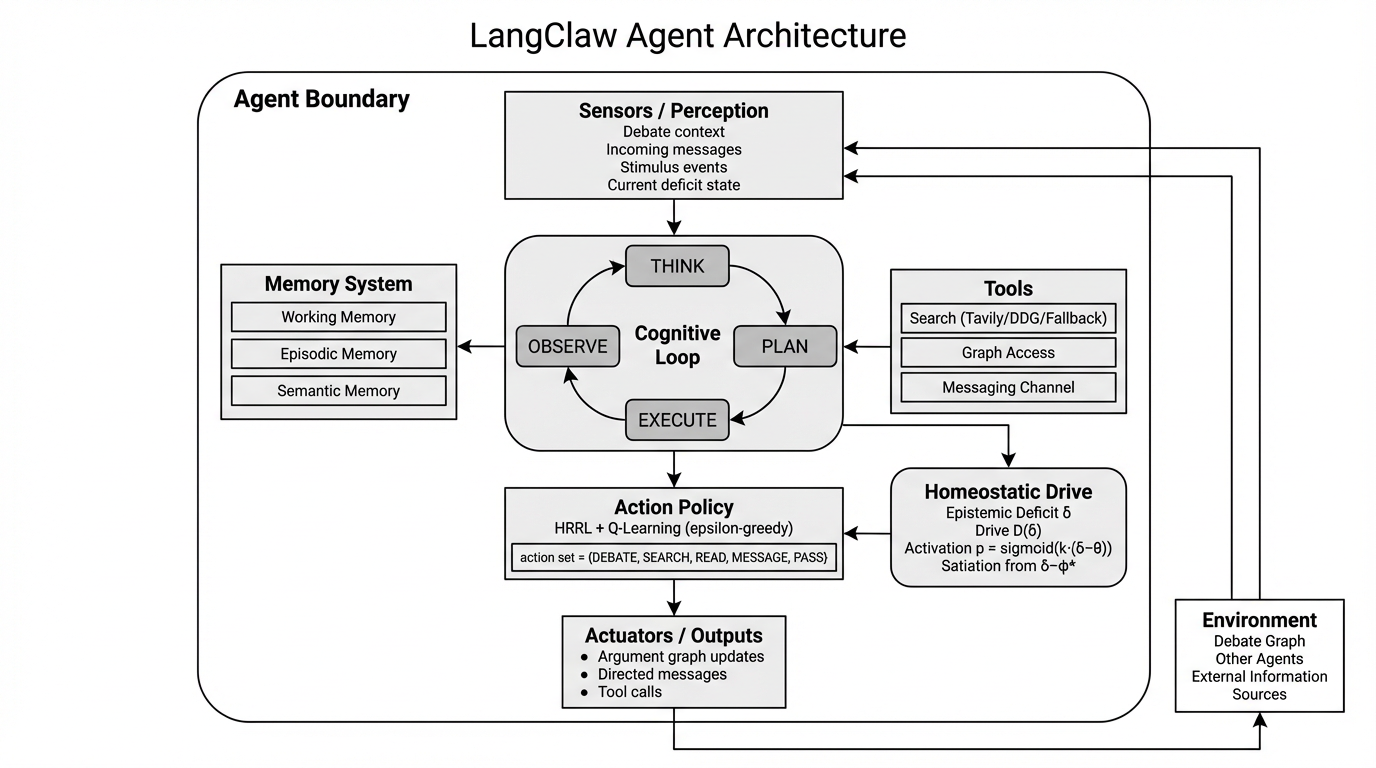
\includegraphics[width=0.86\linewidth]{langclaw/figs/illustration_1.png}
    \caption{Arquitectura del agente LangClaw: lazo cognitivo, memoria,
    herramientas e impulso homeost\'atico.}
    \label{fig:agent_architecture}
\end{figure}

\subsection{Dise\~no del sistema multi-agente}

Del agente al sistema. El tama\~no poblacional responde a un compromiso:
debe ser suficiente para que emerjan din\'amicas sociales, pero acotado
por c\'omputo, tokens y llamadas a la API. Ambas condiciones comparten
diez agentes en dos facciones espejo (Gobierno/Oposici\'on), cada una
con los cinco subsistemas del Modelo de Sistema
Viable~\parencite{beer1972brain} (S1--S5): la \emph{unidad m\'inima
viable} para sostener regulaci\'on individual y observar regulaci\'on
colectiva. La duplicaci\'on espejo introduce el antagonismo de suma cero
(Fig.~\ref{fig:mas_vsm_architecture}).

\begin{figure}[H]
    \centering
    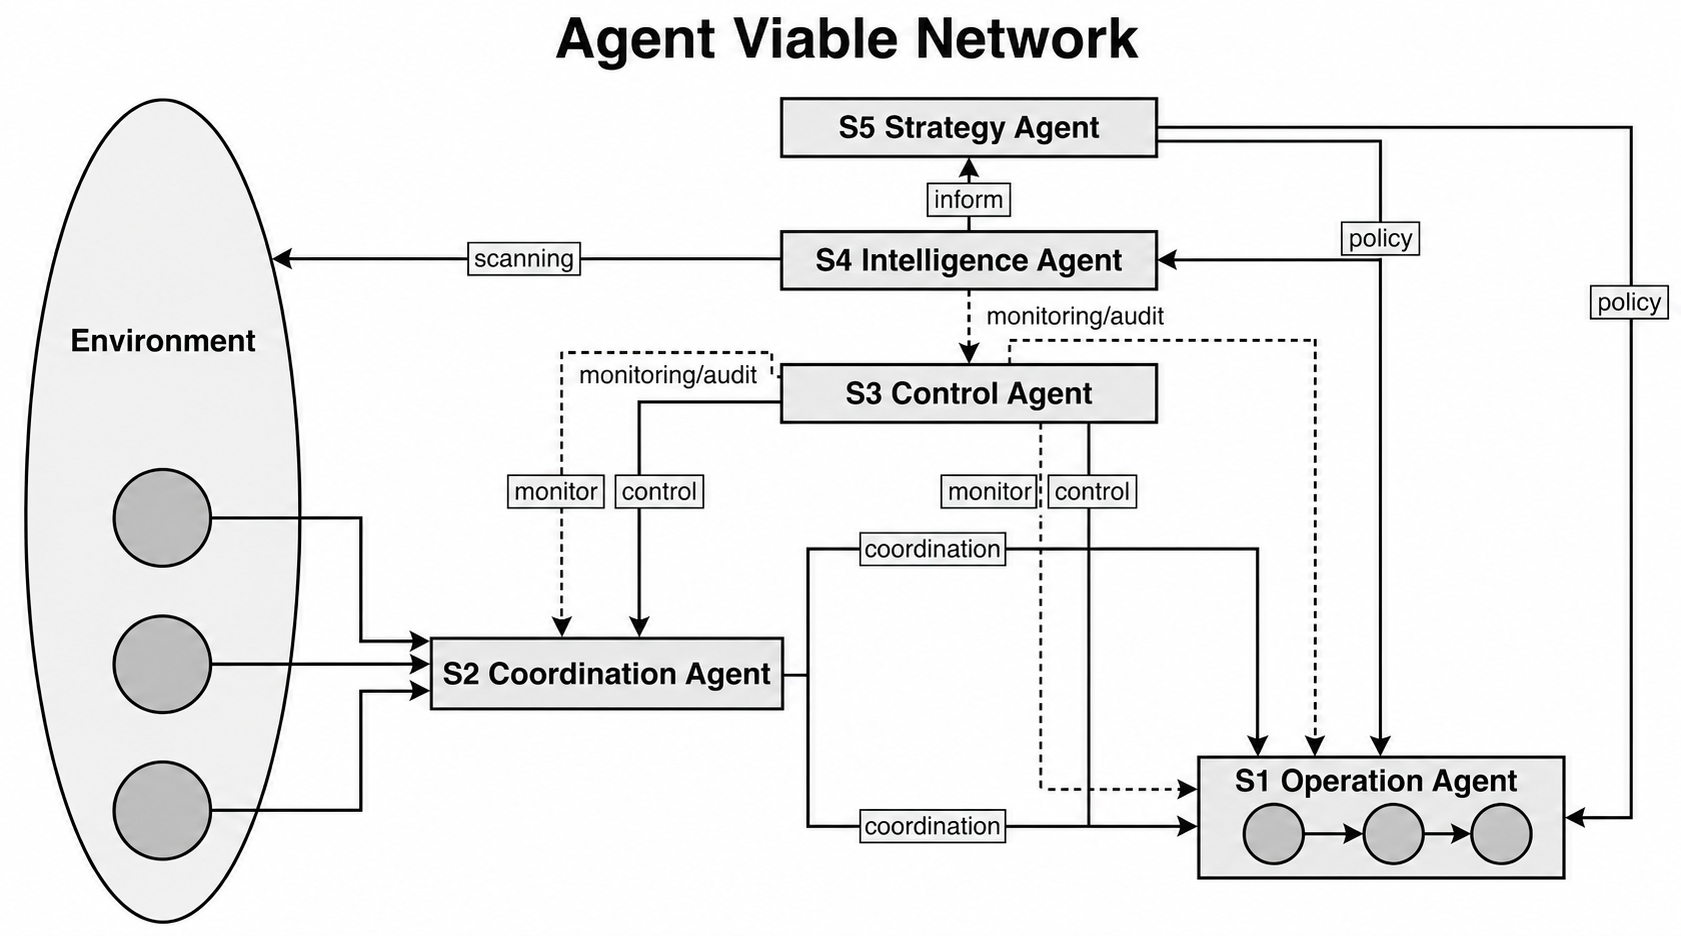
\includegraphics[width=0.90\linewidth]{langclaw/figs/illustration_2.png}
    \caption{Arquitectura multi-agente inspirada en el VSM: organizaci\'on
    faccional espejo y entorno discursivo compartido.}
    \label{fig:mas_vsm_architecture}
\end{figure}

\begin{table}[!t]
\caption{Roles de los subsistemas VSM (espejados en ambas facciones).}
\label{tab:roles}
\small
\begin{tabular}{|l|l|p{6cm}|}
\hline
\textbf{VSM} & \textbf{Rol} & \textbf{Funci\'on principal} \\
\hline
S1 & Operaciones & Producir y defender argumentos; ejecutar tareas de debate. \\
S2 & Coordinaci\'on & Sincronizar acciones aliadas; delegar tareas; enrutar informaci\'on estrat\'egica. \\
S3 & Control & Auditar coherencia interna; detectar contradicciones; enviar mensajes correctivos. \\
S4 & Inteligencia & Escanear al oponente; identificar amenazas; usar SEARCH para recursos externos. \\
S5 & Estrategia & Fijar prioridades; resolver tensiones control--inteligencia; emitir directivas. \\
\hline
\end{tabular}
\end{table}


\subsection{Estrategias de orquestaci\'on}

Agente y sistema definidos, la variable experimental queda aislada: qui\'en
decide cu\'ando act\'ua un agente. Esto permite comparar dos estrategias de
orquestaci\'on bajo capacidades locales equiparables. En la estrategia
propuesta, \textbf{HRRL} (end\'ogena), cada agente regula su ejecuci\'on
mediante la compuerta sigmoide (Ec.~\ref{eq:sigmoid}) y selecciona
acciones v\'ia Q-learning (Ec.~\ref{eq:td0}) con recompensa homeost\'atica.
En la l\'inea base, \textbf{LangGraph} (ex\'ogena), un enrutador LLM decide
qu\'e agente ingresa al lazo cognitivo; el agente seleccionado ejecuta las
mismas capacidades locales. La diferencia no radica en qu\'e pueden hacer
los agentes, sino en d\'onde se resuelve la activaci\'on.

% ============================================================
\section{Dise\~no experimental}
\label{sec:setup}

\subsection{Medidas de desempe\~no e hip\'otesis central}

Definidas ambas estrategias bajo capacidades equiparables, queda
especificar c\'omo distinguirlas emp\'iricamente. Dado que el objetivo
es evaluar autonom\'ia y coherencia argumentativa en el tiempo, las
medidas de desempe\~no m\'as apropiadas son estructurales:
el problema es la organizaci\'on del debate, no la fluidez superficial.
\textbf{Raz\'on de aceptaci\'on AAF}~\parencite{dung1995acceptability}:
$\alpha = \lvert G \rvert / \lvert A \rvert$ (extensi\'on fundamentada sobre
total de argumentos; $\alpha{=}1$: todos no derrotados; $\alpha{=}0$: todos
contestados). \textbf{PRR$_G$}: fracci\'on de debates dirigidos a un nodo
existente~\parencite{anonymous2026madprotocols}. \textbf{$\Delta\varphi^*$}
(Ec.~\ref{eq:phi}): compromiso estructural por intervenci\'on.
\textbf{IR} (verificaci\'on de manipulaci\'on): raz\'on de turnos
homeost\'aticamente activados sobre turnos activos totales; IR${=}1.0$ para
HRRL, ${=}0.0$ para LangGraph. La medida primaria es la
\emph{degradaci\'on temporal}: pendientes de $\Delta\varphi^*$ y $\alpha$
a lo largo de los heartbeats.

\emph{Pregunta de investigaci\'on.} Bajo capacidades locales equiparables
y un horizonte extendido donde el enrutamiento
ex\'ogeno~\parencite{snell2024scaling} ha reportado degradaci\'on,
¿emergen diferencias sistem\'aticas en las trayectorias temporales
de coherencia argumentativa, distribuci\'on de participaci\'on y
calidad estructural entre un r\'egimen de regulaci\'on end\'ogena (HRRL)
y uno de enrutamiento ex\'ogeno (LangGraph)? Formalmente, $H_0$: las
trayectorias no difieren entre condiciones; $H_1$: existen diferencias
atribuibles al mecanismo de activaci\'on. La m\'etrica primaria es la
degradaci\'on temporal; la foto final (Tabla~\ref{tab:results}) es
diagn\'ostico secundario.

El contraste emp\'irico se articula en tres dimensiones: distribuci\'on
de participaci\'on ($\sigma_s$ en ventanas temporales), calidad por
intervenci\'on ($\Delta\varphi^*$ y su pendiente) y coherencia global
del grafo (aceptaci\'on AAF y su pendiente), interpretadas a la luz de
T1 (Sec.~\ref{sec:method}).

\subsection{Configuraci\'on experimental}

\begin{table}
\caption{Hiperpar\'ametros.}\label{tab:hyperparams}
\small
\begin{tabular}{|l|l|l|}
\hline
\textbf{Par\'ametro} & \textbf{S\'imbolo} & \textbf{Valor} \\
\hline
Tasa de decaimiento & $\lambda$ & 0.05 \\
Pendiente sigmoide & $k$ & 10 \\
Umbral de activaci\'on & $\theta$ & 0.7 \\
Tasa de saciedad & $\alpha$ & 3.0 (calibrado de $\{1,2,3\}$) \\
Ganancia de est\'imulo & $\gamma$ & 0.1 \\
L\'inea base / d\'eficit inicial & $\varepsilon$, $\delta_0$ & 0.1, 0.5 \\
Exponente de impulso & $m$ & 2 \\
Tasa de aprendizaje Q & $\eta$ & 0.01 \\
Tasa de exploraci\'on & $\varepsilon_{\text{RL}}$ & 0.1 \\
Factor de descuento & $\gamma_{\text{RL}}$ & 0.95 \\
Pesos de est\'imulo & $(w_F,w_C,w_M,w_N,w_P)$ & $(0.40, 0.15, 0.15, 0.15, 0.15)$ \\
Heartbeats m\'ax / agentes & $T$, $N$ & 80, 10 \\
LLM & --- & GPT-5-nano~\parencite{openai2025gpt5nano} \\
Semillas & $s$ & $\{7,17,42,123,256\}$ \\
\hline
\end{tabular}
\end{table}

\noindent Los par\'ametros del impulso se derivan matem\'aticamente
($\varepsilon{=}0.1$, $m{=}2$:~\textcite{keramati2014homeostatic}) o por
relevancia funcional ($\lambda{=}0.05$: $\sim$14 heartbeats hasta
$\theta$ desde reposo; $\theta{=}0.7$, $k{=}10$, $\gamma_{\text{stim}}{=}0.1$).
Los Q siguen pr\'actica est\'andar TD(0) ($\eta{=}0.01$, $\gamma_{\text{RL}}{=}0.95$,
$\varepsilon_{\text{RL}}{=}0.1$); $\alpha$ y los pesos de est\'imulo se
calibraron emp\'iricamente (Sec.~\ref{sec:setup}).

\subsection{Optimizaci\'on de hiperpar\'ametros}

Los \'unicos par\'ametros sin prior te\'orico ---tasa de saciedad
$\alpha$ y pesos de est\'imulo $(w_F, w_C, w_M, w_N, w_P)$--- se
calibran por ablaci\'on de 15 micro-simulaciones (10 heartbeats HRRL,
$s{=}42$) que cruza cinco perfiles de pesos (\emph{equal},
\emph{faction-dominant} $w_F{=}0.40$, \emph{centrality-dominant},
\emph{novelty-dominant}, \emph{pressure-dominant}) con
$\alpha\in\{1,2,3\}$. La configuraci\'on ganadora ---ordenada por
$\overline{\Delta\varphi^*}$ con consistencia como desempate---
result\'o \emph{faction-dominant}, $\alpha{=}3.0$
($\overline{\Delta\varphi^*}{=}0.136$, consistencia $97.2\%$ en 36
debates), seguida de \emph{novelty-dominant} ($\alpha{=}1$) y
\emph{faction-dominant} ($\alpha{=}2$): duplicar el peso faccional
alinea el sensor con la estructura adversarial y $\alpha$ alto amplifica
la saciedad por unidad de $\Delta\varphi^*$. Las salidas imponen
esquema JSON Pydantic con penalizaci\'on de $+0.1$ tras dos reintentos;
una f\'abrica deriva semillas primas v\'ia SHA-256 para reproducibilidad
y las pruebas usan $t$-test de Welch unilateral con correcci\'on de
Bonferroni.

% ============================================================
\section{Resultados}
\label{sec:results}

\subsection{M\'etricas de resultado}

El heartbeat opera como discretizaci\'on temporal uniforme: ambas
condiciones disponen del mismo n\'umero de tics, mismo horizonte y mismo
presupuesto de tokens y llamadas a la API. La diferencia en
\emph{densidad deliberativa} (debates por heartbeat) refleja, por
construcci\'on, capacidad end\'ogena de auto-activaci\'on bajo presi\'on
epist\'emica, no un ajuste de presupuesto. La comparaci\'on de calidad
se realiza, en consecuencia, sobre m\'etricas estructurales normalizadas
por intervenci\'on ($\overline{\Delta\varphi^*}$, aceptaci\'on AAF,
PRR$_G$), de modo que diferencias en densidad no contaminen la
comparaci\'on de coherencia agregada.

\begin{table}
\caption{Resultados preliminares (n${=}3$ pares de semillas $\{7,17,42\}$,
$T=80$ heartbeats). Filas con ${}^\dagger$: media $\pm$ desviaci\'on
(muestral); restantes corresponden a la semilla 7 representativa, a la
espera del cierre de las semillas 123 y 256. Las m\'etricas de calidad
est\'an normalizadas por intervenci\'on.}\label{tab:results}
\small
\begin{tabular}{|l|c|c|}
\hline
\textbf{M\'etrica} & \textbf{HRRL} & \textbf{LangGraph} \\
\hline
Total debates${}^\dagger$  & $387.0 \pm 3.0$ & $69.3 \pm 6.7$ \\
Densidad deliberativa (deb./hb.) & 4.84 & 0.87 \\
Nodos / aristas (s.\ 7)    & 390 / 384 & 71 / 70 \\
\hline
$\sigma_s$ por agente (\textbf{H}; s.\ 7) & 4.65 & 8.30 \\
Agentes con 0 debates (s.\ 7) & 0 / 10 & 3 / 10 \\
\hline
Raz\'on de aceptaci\'on AAF${}^\dagger$ & $0.681 \pm 0.010$ & $0.540 \pm 0.029$ \\
PRR$_G$ (s.\ 7)            & 0.990 & 0.986 \\
$\overline{\Delta\varphi^*}$ por debate (s.\ 7) & 0.142 & 0.092 \\
\hline
Pendiente $\Delta\varphi^*$ (s.\ 7) & $+$0.018 & $-$0.016 \\
Pendiente aceptaci\'on (s.\ 7) & $+$0.018 & $-$0.002 \\
\hline
IR (verificaci\'on)        & 1.0 & 0.0 \\
Recompensa media${}^\dagger$ & $-1.85 \pm 0.15$ & $+0.42 \pm 0.08$ \\
\hline
\end{tabular}
\end{table}

La primera verificaci\'on es estructural: IR${}=1.0$ para HRRL y
$0.0$ para LangGraph confirma que las condiciones son funcionalmente
distintas. La Tabla~\ref{tab:results} presenta resultados preliminares
de los tres primeros pares de semillas $\{7, 17, 42\}$; las restantes
($\{123, 256\}$) est\'an en ejecuci\'on y los promedios y pruebas se
actualizar\'an al cierre. A continuaci\'on se interrogan los datos.

\textbf{¿Qui\'en habla?}
T1 predice activaci\'on sostenida en todo agente con $\delta_i > \varepsilon$;
aplicada a una poblaci\'on con impulsos sim\'etricos, implica distribuci\'on
emergente de la participaci\'on: el impulso acumulado empuja a actuar a
quien se silencia. Los datos bajo HRRL son
consistentes: los 10 agentes debaten (rango 31--47, $\sigma_s = 4.65$).
Bajo LangGraph, donde ese mecanismo no opera, 3 agentes no intervienen
y uno concentra el 38\% de los debates ($\sigma_s = 8.30$); los
silenciados acumulan d\'eficits de 7.5--7.8 ($\sim$10$\times\theta$) que
el enrutador no corrige.

\textbf{¿La cantidad sacrifica calidad?}
Bajo el mismo presupuesto temporal, HRRL exhibe $5.5\times$ mayor
densidad deliberativa (4.88 vs 0.89 debates por heartbeat). La pregunta
relevante no es si genera m\'as, sino si esa densidad degrada la
calidad agregada por intervenci\'on. La respuesta es negativa:
$\overline{\Delta\varphi^*}$ por debate es superior (0.142 vs 0.092),
y la trayectoria temporal mejora en HRRL ($+0.018$ por ventana) mientras
LangGraph se degrada ($-0.016$). El enrutador se agota; la regulaci\'on
end\'ogena sostiene calidad mientras escala densidad.

\textbf{¿M\'as argumentos implican m\'as refutaci\'on?}
Intuitivamente, quintuplicar los debates deber\'ia reducir la aceptaci\'on.
Ocurre lo contrario (0.687 vs 0.563): bajo HRRL crece monot\'onicamente
($0.62 \to 0.69$); LangGraph se estanca en $0.57$. La participaci\'on
distribuida no degrada la estructura del grafo: la fortalece.

\textbf{¿Opera el mecanismo en su r\'egimen te\'orizado?}
No plenamente: la recompensa media bajo HRRL es negativa y consistente
entre semillas ($-1.85 \pm 0.15$, n${=}3$); en LangGraph se mantiene
positiva ($+0.42 \pm 0.08$). En HRRL los d\'eficits finales muestran
adem\'as asimetr\'ia faccional (GOV: 13--20; OPP: 0.1--6.1, semilla 7).
La calibraci\'on de $\alpha$ se hizo antes de activar la difusi\'on
completa de eventos y qued\'o sub-dimensionada para el flujo real
(Sec.~\ref{sec:setup}). Las m\'etricas macro mejoran aun bajo este
r\'egimen sub\'optimo, sugiriendo robustez del efecto emergente.

\textbf{¿Se puede confiar en estos patrones?}
Con $n{=}3$ la potencia inferencial es limitada, pero la consistencia
direccional es estricta: los tres pares favorecen a HRRL en debates,
aceptaci\'on AAF y distribuci\'on de participaci\'on. Wilcoxon
signed-rank pareado arroja $p{=}0.25$ ---l\'imite te\'orico para $n{=}3$
con todos los signos alineados--- por lo que el test no rechaza $H_0$
pero tampoco compite con la se\~nal. La prueba formal de Welch
unilateral con Bonferroni se completar\'a con las cinco semillas; la
coherencia entre m\'etricas estructuralmente independientes y su
alineaci\'on con \textsc{T1} reducen la probabilidad de artefacto.

% ============================================================
\section{Discusi\'on}
\label{sec:discussion}

\subsection{Interpretaci\'on de los resultados}

\textbf{Mec\'anica.} El impulso (Ec.~\ref{eq:reward}) crece en todo
agente inactivo y la compuerta sigmoide (Ec.~\ref{eq:sigmoid}) dispara
cuando $\delta_i > \theta$: el balance ($\sigma_s$: 4.65 vs 8.30)
emerge de la simetr\'ia del impulso, no fue dise\~nado. La
concentraci\'on bajo LangGraph evoca la oligarqu\'ia de
Michels~\parencite{michels1911political}.

\textbf{Emergencia.} Quintuplicar la actividad \emph{fortalece} el grafo
($\alpha$: 0.687 vs 0.563): la diversidad de atacantes estabiliza la
extensi\'on fundamentada, an\'alogo a la variedad
requerida~\parencite{ashby1956introduction}. Foto y pendiente favorecen
a HRRL en $\Delta\varphi^*$ ($0.142$ vs $0.092$; $+0.018$ vs $-0.016$);
medir \emph{procesos}~\parencite{snell2024scaling} captura din\'amicas
que la foto final oculta.

El \emph{mecanismo} fue dise\~nado ex\'ogenamente; lo end\'ogeno es la
\emph{din\'amica} que emerge una vez instanciada, aunque el r\'egimen
oscilatorio predicho requiere recalibraci\'on bajo el flujo real.

\textbf{Limitaciones.} $n{=}5$ semillas es exploratorio aunque los
efectos son grandes; la calibraci\'on us\'o una sola semilla y un flujo
de est\'imulos menor al r\'egimen final, dejando $\alpha$ sub-dimensionado
(recompensa negativa bajo HRRL); los pesos Q son adaptativos, no una
pol\'itica convergida; los pesos de $\Delta\varphi^*$ son prior
principiado sin validaci\'on; resultados espec\'ificos a GPT-5-nano; el
mecanismo podr\'ia ser explotado por argumentos estructuralmente bien
ubicados pero sem\'anticamente vac\'ios.

\textbf{Trabajo futuro.} (i)~formalizar la paradoja de la aceptaci\'on
buscando un umbral de diversidad de atacantes que estabilice la
extensi\'on fundamentada; (ii)~integrar DeLP~\parencite{garcia2004defeasible}
para garant\'ias y derrotabilidad expl\'icita; (iii)~validaci\'on
cruzada de la calibraci\'on, sensibilidad de $\theta,\alpha,\lambda$,
escalamiento poblacional y presupuestos restringidos~\parencite{snell2024scaling};
y (iv)~validaci\'on externa LLM-as-judge con r\'ubrica multi-criterio
de pesos derivados por AHP~\parencite{saaty1980ahp,lu2024ahp}, dos
jueces independientes (Claude Opus, Gemini Pro) bajo evaluaci\'on
ciega con Krippendorff $\alpha$ ordinal como fiabilidad inter-juez.

% ============================================================
\section{Conclusiones}
\label{sec:conclusion}

LangClaw pregunta si el colapso del contexto en debate multi-agente LLM
se aborda mejor por planificaci\'on externa o regulaci\'on end\'ogena.
Bajo presupuesto temporal equiparable, los resultados preliminares
muestran que HRRL exhibe mayor densidad deliberativa y sostiene mejor
coherencia estructural agregada que LangGraph; la calidad por
intervenci\'on mejora en el tiempo y la participaci\'on se distribuye
sin enrutador externo. El hallazgo m\'as inesperado ---el aumento
monot\'onico de aceptaci\'on pese a mayor densidad--- sugiere que la
diversidad de participaci\'on puede estabilizar la estructura
argumentativa a\'un bajo calibraci\'on sub\'optima. El aporte es
tambi\'en metodol\'ogico: una forma testeable de preguntar si la
coherencia en MAS puede ser propiedad autoorganizada.

% ============================================================
\section*{Reproducibilidad}

C\'odigo e instrucciones de reproducibilidad:
\url{https://github.com/pgerpe/langclaw_experiment}

\printbibliography

\end{document}
